\documentclass[11pt,a4paper]{article}

\usepackage[utf8]{inputenc}
\usepackage[T1]{fontenc}
\usepackage[french]{babel}
\usepackage{geometry}
\usepackage[table]{xcolor}
\usepackage{array}
\usepackage{tabularx}
\usepackage{enumitem}
\usepackage{listings}
\usepackage{hyperref}
\usepackage{fancyhdr}
\usepackage{titlesec}
\usepackage{graphicx}
\usepackage{float}

\geometry{margin=2.1cm}
\definecolor{codebg}{RGB}{245,247,250}
\definecolor{blue}{RGB}{30,75,130}

\hypersetup{colorlinks=true,linkcolor=blue,urlcolor=blue}
\pagestyle{fancy}
\fancyhf{}
\lhead{Les tests continus}
\rhead{TP : Les tests continus dans DevOps}
\cfoot{\thepage}
\titleformat{\section}{\large\bfseries\color{blue}}{\thesection.}{0.5em}{}
\setlist[itemize]{leftmargin=1.1cm,itemsep=2pt}
\setlist[enumerate]{leftmargin=1.1cm,itemsep=2pt}

\lstdefinestyle{project}{
    basicstyle=\ttfamily\small,
    backgroundcolor=\color{codebg},
    frame=single,
    rulecolor=\color{gray!35},
    columns=fullflexible,
    keepspaces=true,
    showstringspaces=false,
    breaklines=true
}

\begin{document}

\begin{center}
{\large\bfseries Université Ibn Khaldoun de Tiaret}\\[2pt]
{\normalsize Département de Mathématiques et d'Informatique}\\[5pt]
{\normalsize Master Sécurité informatique}\\[2pt]
{\normalsize Module : DevOps}\\[9pt]
\rule{0.9\textwidth}{0.5pt}\\[9pt]
{\Large\bfseries FICHE DE TP}\\[5pt]
{\LARGE\bfseries Les tests continus dans DevOps}\\[7pt]
{\large Application simplifiée de gestion intelligente de l'énergie solaire}\\[10pt]
\begin{tabular}{rl}
\textbf{Enseignant :} & Abdelkader Ouared\\
\textbf{Outils :} & Git, GitHub, Pytest et GitHub Actions
\end{tabular}\\[8pt]
\rule{0.9\textwidth}{0.5pt}
\end{center}

\section{Objectif}

Tester une petite application Python qui surveille une installation solaire, puis
lancer ces tests automatiquement avec \textbf{GitHub Actions}. Le code est simple
et les messages IoT sont simulés avec des données Python : l'important est de
\textbf{comprendre la démarche}, pas d'écrire beaucoup de code.

\section{Contexte}

Une maison possède des panneaux solaires, une batterie et trois capteurs IoT
(S1 : production en W, S2 : consommation en W, S3 : niveau de batterie en \%).
L'application reçoit leurs messages et génère une alerte si la batterie est faible
ou si une mesure est invalide (figure~\ref{fig:contexte}).

\begin{figure}[!htbp]
\centering
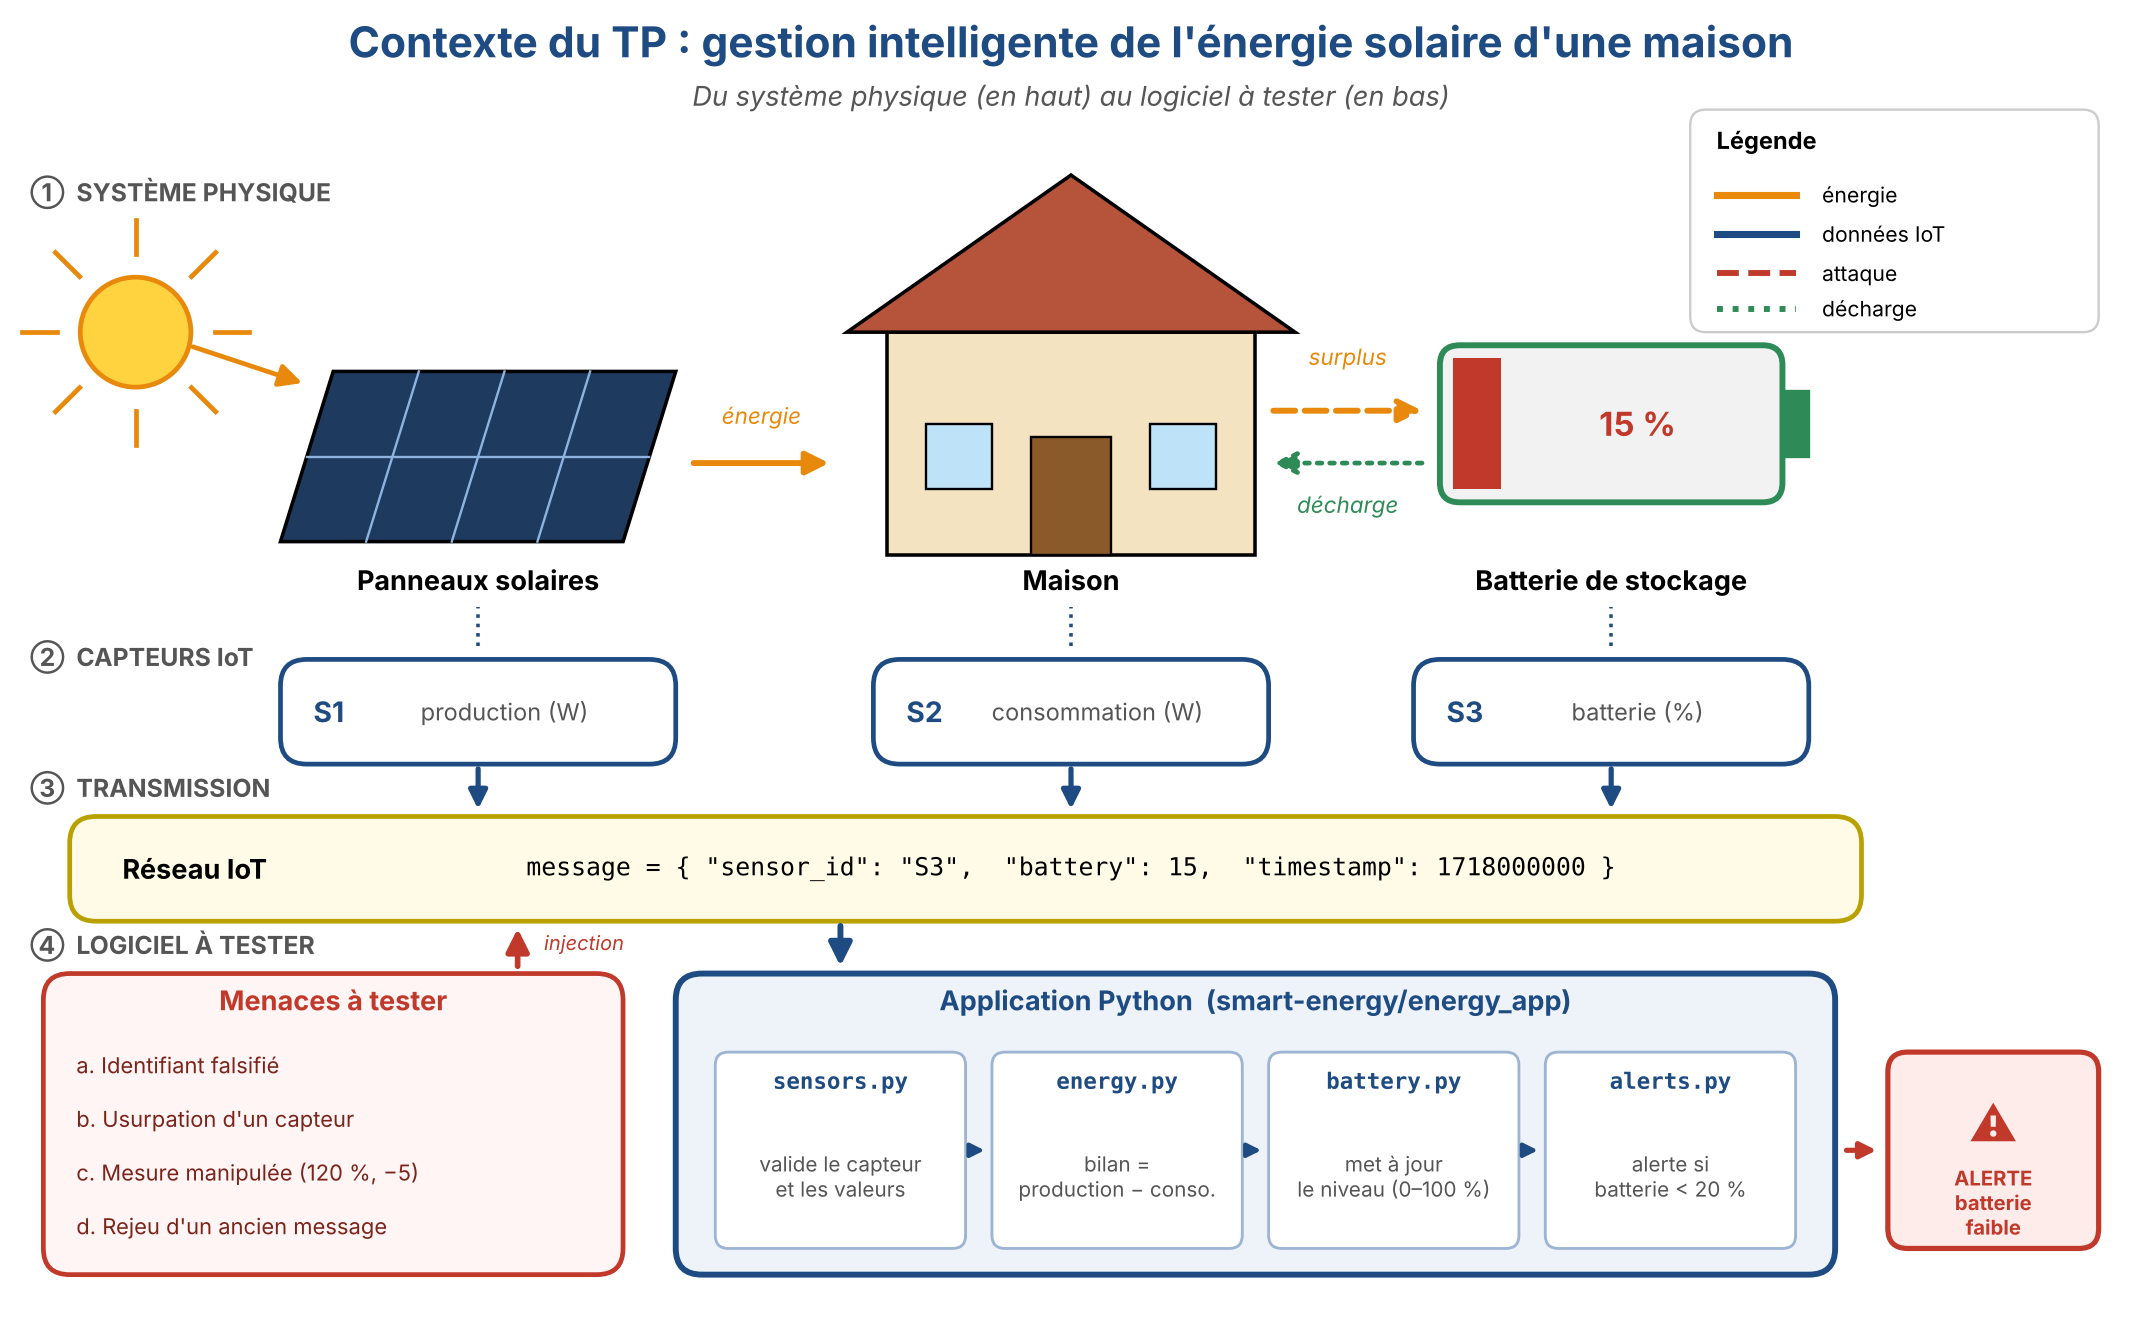
\includegraphics[width=0.9\textwidth]{contexte_energie_intelligente_v2.png}
\caption{Le système réel : du matériel aux capteurs, au réseau, puis à l'application à tester.}
\label{fig:contexte}
\end{figure}

\textbf{Règles à respecter :}
batterie entre 0 et 100~\% ; production et consommation jamais négatives ;
capteur à identifiant connu ; alerte si batterie sous 20~\% ; surplus de production
utilisable pour charger la batterie.

\textbf{Aspect sécurité :} les identifiants des capteurs ne sont \textbf{pas stockés en clair}.
Le registre \texttt{energy\_app/data/sensors.json} ne contient que leur \textbf{empreinte
(hash SHA-256 avec un sel)}, associée à la mesure que le capteur a le droit d'envoyer.
À la réception d'un message, l'application hache l'identifiant reçu et cherche
cette empreinte dans le fichier JSON.

\section{Structure du projet}

\begin{lstlisting}[style=project]
smart-energy/
|-- energy_app/           : sensors.py, energy.py, battery.py, alerts.py
|   `-- data/sensors.json : registre des capteurs (identifiants haches)
|-- tests/                : test_sensors.py, test_energy.py, test_battery.py,
|                           test_alerts.py, test_integration.py,
|                           test_security.py
|-- .github/workflows/    : tests.yml
|-- requirements.txt, .gitignore, README.md
\end{lstlisting}

\paragraph{Projet fourni (archive \texttt{smart-energy.zip}).}
Le squelette est donné : les fichiers de \texttt{tests/} sont \textbf{vides} (c'est à vous de
les écrire) et certains modules sont à compléter aux endroits marqués \texttt{TODO}.

\begin{center}
\footnotesize
\renewcommand{\arraystretch}{1.2}
\begin{tabularx}{\textwidth}{|>{\ttfamily}p{3.4cm}|p{1.8cm}|X|}
\hline
\rowcolor{blue!12} \textrm{Fichier} & \textrm{État} & \textrm{À compléter}\\
\hline
energy.py & complet & rien (sert d'exemple)\\
\hline
sensors.py & partiel & vérification d'usurpation (\texttt{SensorMismatchError}) ; \texttt{ReplayGuard.check} (\texttt{ReplayError})\\
\hline
data/sensors.json & fourni & registre JSON des identifiants hachés (ne pas modifier)\\
\hline
battery.py & partiel & \texttt{update\_level}\\
\hline
alerts.py & partiel & \texttt{battery\_alert}\\
\hline
tests/*.py & vides & écrire les tests (section~\ref{sec:liste})\\
\hline
tests.yml & partiel & les 4 \texttt{TODO} du fichier\\
\hline
\end{tabularx}
\end{center}

\noindent\textbf{Format d'un message IoT :}
\texttt{sensor\_id}, \texttt{timestamp} et une seule mesure parmi \texttt{production},
\texttt{consumption}, \texttt{battery}. Capteurs connus : S1 (\texttt{production}),
S2 (\texttt{consumption}), S3 (\texttt{battery}). Toutes les erreurs de message héritent de
\texttt{InvalidMeasurement}, qui est un \texttt{ValueError}.

\noindent\textbf{Registre haché.} Dans \texttt{sensors.py}, \texttt{hash\_sensor\_id(sensor\_id, salt)} calcule
l'empreinte SHA-256 de \texttt{sel + identifiant} et \texttt{load\_registry()} lit le fichier JSON.
Le script \texttt{scripts/generate\_registry.py} permet de régénérer le registre.

\section{Travail demandé}

\textit{Conseil : avancez étape par étape. Un test simple qui fonctionne vaut mieux
qu'un test compliqué qui ne marche pas.}

\subsection{Comprendre les modules}

Expliquer en une phrase le rôle de \texttt{sensors.py}, \texttt{energy.py},
\texttt{battery.py} et \texttt{alerts.py}, et dire quelles données passent de l'un à l'autre.

\subsection{Tests unitaires}

Pour chaque module, écrire \textbf{un test normal} et \textbf{un test d'erreur}.
Voir la liste détaillée (section~\ref{sec:liste}). Idées : capteur connu / inconnu ; batterie à 15~\% / à 120~\% ;
production supérieure à la consommation / valeur négative.

\subsection{Tests d'intégration}

Écrire \textbf{deux tests} qui font travailler plusieurs modules ensemble
(par exemple : mesure reçue $\rightarrow$ bilan $\rightarrow$ batterie, ou batterie
faible $\rightarrow$ alerte). Il existe deux façons d'assembler les modules :

\begin{center}
\renewcommand{\arraystretch}{1.25}
\begin{tabularx}{\textwidth}{|>{\bfseries}p{3.2cm}|X|}
\hline
Ascendante (bottom-up) & On teste d'abord les petits modules, puis on les assemble de proche en proche.\\
\hline
Descendante (top-down) & On part du scénario complet, en remplaçant par des simulacres les modules pas encore intégrés.\\
\hline
\end{tabularx}
\end{center}

Indiquer pour chaque test la méthode que vous avez utilisée (scénarios proposés en section~\ref{sec:liste}).

\subsection{Tests de sécurité}

Un test qui passe prouve que le code respecte la règle \emph{écrite}, pas que la règle
protège vraiment. Exemple : règle \og bloquer une IP après 3 échecs \fg{}.
Test : 3 mauvais mots de passe depuis la même IP $\rightarrow$ IP bloquée, le test passe.
Mais un attaquant qui essaie 1 mot de passe depuis chacune de 10 IP n'est jamais bloqué :
la règle est insuffisante.

Compléter le tableau suivant \textbf{en une phrase par case} :

\begin{center}
\renewcommand{\arraystretch}{1.3}
\begin{tabularx}{\textwidth}{|p{3.6cm}|X|X|}
\hline
\rowcolor{blue!12} Menace & Entrée malveillante et résultat attendu (test) & La règle suffit-elle ? Pourquoi ?\\
\hline
Identifiant falsifié (capteur inconnu) & \rule{0pt}{1.2cm} &\\
\hline
Usurpation (S1 se fait passer pour S3) & \rule{0pt}{1.2cm} &\\
\hline
Mesure manipulée (batterie à 120~\%) & \rule{0pt}{1.2cm} &\\
\hline
Rejeu (ancien message renvoyé) & \rule{0pt}{1.2cm} &\\
\hline
Fichier JSON lu par un attaquant (identifiants hachés) & \rule{0pt}{1.2cm} &\\
\hline
\end{tabularx}
\end{center}

Écrire des tests Pytest pour \textbf{au moins trois} de ces menaces (section~\ref{sec:liste}).

\textbf{Question sur le registre haché :} un attaquant qui lit \texttt{sensors.json} peut-il retrouver
l'identifiant \texttt{S1} ? Que se passe-t-il si les identifiants sont courts et faciles à deviner ?
Que faudrait-il changer (identifiants longs et aléatoires, clé secrète) ?

\subsection{GitHub Actions}

Créer \texttt{.github/workflows/tests.yml} : à chaque \texttt{push} et
\texttt{pull\_request} sur \texttt{main}, récupérer le code, installer Python,
installer \texttt{requirements.txt} et lancer \texttt{pytest -v}.

\section{Liste détaillée des tests à écrire}\label{sec:liste}

Cette liste correspond au projet fourni. Les tests marqués \textbf{obl.} sont
obligatoires (\textbf{13 tests} au total, ce qui couvre les minimums demandés) ; les tests
\textbf{bonus} permettent d'aller plus loin. Pour chaque test : \emph{situation $\rightarrow$
résultat attendu}.

\newcommand{\tabhead}[1]{\multicolumn{4}{|l|}{\cellcolor{blue!12}\textbf{#1}}\\\hline}
\footnotesize
\renewcommand{\arraystretch}{1.25}

\paragraph{Tests unitaires.}
\begin{center}
\begin{tabularx}{\textwidth}{|>{\bfseries}p{0.8cm}|X|X|p{1cm}|}
\hline
\tabhead{\texttt{tests/test\_sensors.py} (fonctions \texttt{parse\_measurement}, \texttt{hash\_sensor\_id})}
S1 & Capteur connu, mesure valide : S3 envoie \texttt{battery} = 15 & mesure retournée (\texttt{metric} = \texttt{battery}, \texttt{value} = 15) & obl.\\\hline
S2 & S1 envoie \texttt{production} = 1200 & \texttt{metric} = \texttt{production}, \texttt{value} = 1200 & bonus\\\hline
S3 & Identifiant inconnu \texttt{S99} & \texttt{UnknownSensorError} & obl.\\\hline
S4 & Message sans \texttt{timestamp} & \texttt{InvalidMeasurement} & bonus\\\hline
S5 & Valeur non numérique (texte \texttt{abc}) & \texttt{InvalidMeasurement} & bonus\\\hline
S6 & Deux mesures dans le même message & \texttt{InvalidMeasurement} & bonus\\\hline
S7 & Hachage : \texttt{hash\_sensor\_id} pour S1 (deux appels) puis pour S2 & empreinte de 64 caractères, différente de \texttt{S1}, identique entre les deux appels, différente pour S2 & bonus\\\hline
\tabhead{\texttt{tests/test\_energy.py} (fonctions \texttt{compute\_balance}, \texttt{has\_surplus})}
E1 & Production 1200 W, consommation 800 W & bilan = 400, surplus vrai & obl.\\\hline
E2 & Production 300 W, consommation 900 W & bilan = $-600$, surplus faux & bonus\\\hline
E3 & Production négative ($-100$) & \texttt{ValueError} & obl.\\\hline
E4 & Consommation négative ($-1$) & \texttt{ValueError} & bonus\\\hline
\tabhead{\texttt{tests/test\_battery.py} (fonctions \texttt{validate\_level}, \texttt{is\_low}, \texttt{update\_level})}
B1 & Niveau 15~\% & \texttt{is\_low} vrai & obl.\\\hline
B2 & Niveau 50~\% puis 20~\% (limite) & \texttt{is\_low} faux dans les deux cas & bonus\\\hline
B3 & Niveau 120~\% puis $-5$ & \texttt{ValueError} & obl.\\\hline
B4 & Niveau 50~\%, bilan +500 W pendant 1 h (capacité 5000 Wh) & nouveau niveau = 60 & bonus\\\hline
B5 & Niveau 99~\%, bilan +5000 W pendant 1 h & niveau plafonné à 100 & bonus\\\hline
B6 & Niveau 5~\%, bilan $-2000$ W pendant 1 h & niveau plancher à 0 & bonus\\\hline
\tabhead{\texttt{tests/test\_alerts.py} (fonctions \texttt{battery\_alert}, \texttt{invalid\_measurement\_alert})}
A1 & Niveau 15~\% & alerte de type \texttt{BATTERIE\_FAIBLE} & obl.\\\hline
A2 & Niveau 80~\% & aucune alerte (\texttt{None}) & bonus\\\hline
A3 & Niveau 120~\% & \texttt{ValueError} & obl.\\\hline
A4 & Erreur \texttt{capteur inconnu} & alerte de type \texttt{MESURE\_INVALIDE} & bonus\\\hline
\end{tabularx}
\end{center}

\paragraph{Tests d'intégration} (\texttt{tests/test\_integration.py}).
\begin{center}
\begin{tabularx}{\textwidth}{|>{\bfseries}p{0.8cm}|X|X|p{2.3cm}|}
\hline
I1 & Messages S1 (\texttt{production} = 1200) et S2 (\texttt{consumption} = 800) $\rightarrow$ bilan & bilan = 400 W & ascendante, obl.\\\hline
I2 & Bilan de +500 W, batterie à 50~\% $\rightarrow$ mise à jour du niveau & niveau = 60 & ascendante, bonus\\\hline
I3 & Message S3 avec \texttt{battery} = 15 $\rightarrow$ lecture du message $\rightarrow$ alerte & alerte \texttt{BATTERIE\_FAIBLE} & descendante, obl.\\\hline
I4 & Message de S99 $\rightarrow$ erreur $\rightarrow$ alerte & alerte \texttt{MESURE\_INVALIDE} & descendante, bonus\\\hline
\end{tabularx}
\end{center}

\paragraph{Tests de sécurité} (\texttt{tests/test\_security.py}, fichier à remplir ; X1 à X3 obligatoires, X4 à X6 bonus).
\begin{center}
\begin{tabularx}{\textwidth}{|>{\bfseries}p{0.8cm}|X|X|p{1cm}|}
\hline
X1 & Identifiant falsifié : message du capteur \texttt{S99} & \texttt{UnknownSensorError} & obl.\\\hline
X2 & Usurpation : S1 envoie une mesure \texttt{battery} & \texttt{SensorMismatchError} (échoue tant que le \texttt{TODO} de \texttt{sensors.py} n'est pas fait) & obl.\\\hline
X3 & Mesure manipulée : \texttt{battery} = 120, puis $-5$ & \texttt{ValueError} & obl.\\\hline
X4 & Rejeu : \texttt{ReplayGuard.check} appelé deux fois avec le même horodatage, puis avec un horodatage plus ancien & \texttt{ReplayError} (échoue tant que \texttt{ReplayGuard.check} n'est pas complété) & bonus\\\hline
X5 & Le hash de S3 est envoyé à la place de l'identifiant & \texttt{UnknownSensorError} (une empreinte n'est pas un identifiant) & bonus\\\hline
X6 & Lecture du texte de \texttt{sensors.json} & aucun identifiant en clair (\texttt{S1}, \texttt{S2}, \texttt{S3}) dans le fichier & bonus\\\hline
\end{tabularx}
\end{center}
\normalsize

\textbf{Remarques :}
les tests B4 à B6 et I2 nécessitent de compléter \texttt{update\_level} ; A1, I3 et I4 nécessitent
\texttt{battery\_alert}. X5 et S7 utilisent le registre fourni (pour X5 : \texttt{load\_registry()} donne le sel, \texttt{hash\_sensor\_id} calcule l'empreinte). Un test de sécurité qui échoue au départ est normal : il révèle
une faille à corriger dans le code.

\section{Commandes utiles}

\begin{lstlisting}[style=project]
pip install -r requirements.txt     # installer les dependances
pytest -v                           # lancer tous les tests
pytest -v tests/test_battery.py     # lancer un seul fichier
\end{lstlisting}

\section{À remettre}

\begin{enumerate}
    \item le projet (modules et tests unitaires, d'intégration et de sécurité) ;
    \item le tableau de sécurité rempli ;
    \item le fichier \texttt{tests.yml} ;
    \item le lien du dépôt GitHub et une capture du workflow.
\end{enumerate}

\section{Barème indicatif}

\begin{center}
\begin{tabular}{|p{10cm}|c|}
\hline
\textbf{Critère} & \textbf{Points}\\
\hline
Décomposition et organisation du projet & 3\\
Tests unitaires & 5\\
Tests d'intégration & 3\\
Tests de sécurité & 4\\
Configuration GitHub Actions & 3\\
Documentation et dépôt GitHub & 2\\
\hline
\textbf{Total} & \textbf{20}\\
\hline
\end{tabular}
\end{center}

\section{Question finale}

Pourquoi faut-il vérifier l'identifiant d'un capteur IoT et la cohérence de ses mesures
avant de les utiliser pour gérer l'énergie ?

\end{document}
